\documentclass{article}
\usepackage{tikz}
\usepackage{skak} 
\usetikzlibrary{arrows,automata}
\usetikzlibrary{positioning}

\pagestyle{empty}

\begin{document}
Bill Davis\\
Homework 2

\begin{enumerate}
  \item [1]
  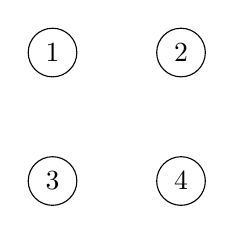
\begin{tikzpicture} [every node/.style={draw,circle}]
\node (a) {1};
\node (b) [right=of a] {2};
\node (c) [below=of a] {3};
\node (d) [right=of c] {4};
      
\end{tikzpicture}
  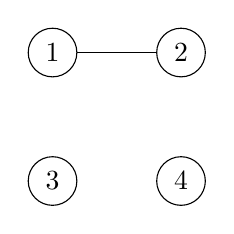
\begin{tikzpicture} [every node/.style={draw,circle}]
\node (a) {1};
\node (b) [right=of a] {2};
\node (c) [below=of a] {3};
\node (d) [right=of c] {4};
 
\draw[-](a)--(b);
     
\end{tikzpicture}
  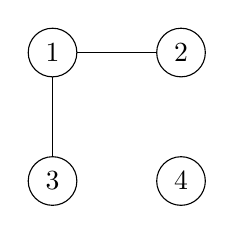
\begin{tikzpicture} [every node/.style={draw,circle}]
\node (a) {1};
\node (b) [right=of a] {2};
\node (c) [below=of a] {3};
\node (d) [right=of c] {4};
 
\draw[-](a)--(b);
\draw[-](a)--(c);
\end{tikzpicture}   
  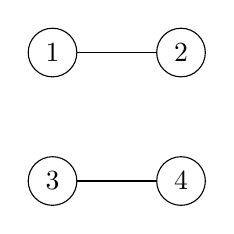
\begin{tikzpicture} [every node/.style={draw,circle}]
\node (a) {1};
\node (b) [right=of a] {2};
\node (c) [below=of a] {3};
\node (d) [right=of c] {4};
 
\draw[-](a)--(b);
\draw[-](c)--(d);
\end{tikzpicture}

  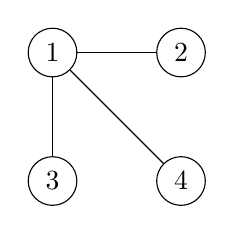
\begin{tikzpicture} [every node/.style={draw,circle}]
\node (a) {1};
\node (b) [right=of a] {2};
\node (c) [below=of a] {3};
\node (d) [right=of c] {4};
 
\draw[-](a)--(b);
\draw[-](a)--(c);
\draw[-](a)--(d);
\end{tikzpicture} 
  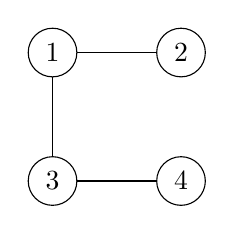
\begin{tikzpicture} [every node/.style={draw,circle}]
\node (a) {1};
\node (b) [right=of a] {2};
\node (c) [below=of a] {3};
\node (d) [right=of c] {4};
 
\draw[-](a)--(b);
\draw[-](c)--(d);
\draw[-](a)--(c);
\end{tikzpicture}
  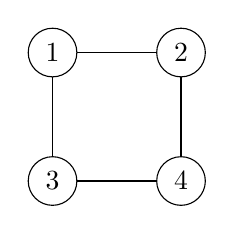
\begin{tikzpicture} [every node/.style={draw,circle}]
\node (a) {1};
\node (b) [right=of a] {2};
\node (c) [below=of a] {3};
\node (d) [right=of c] {4};
 
\draw[-](a)--(b);
\draw[-](c)--(d);
\draw[-](a)--(c);
\draw[-](d)--(b);
\end{tikzpicture}      
   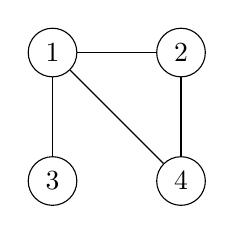
\begin{tikzpicture} [every node/.style={draw,circle}]
\node (a) {1};
\node (b) [right=of a] {2};
\node (c) [below=of a] {3};
\node (d) [right=of c] {4};
 
\draw[-](a)--(b);
\draw[-](a)--(c);
\draw[-](a)--(d);
\draw[-](b)--(d);
\end{tikzpicture}     	
   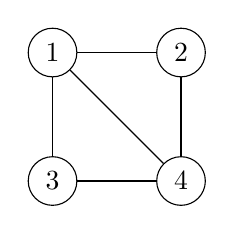
\begin{tikzpicture} [every node/.style={draw,circle}]
\node (a) {1};
\node (b) [right=of a] {2};
\node (c) [below=of a] {3};
\node (d) [right=of c] {4};
 
\draw[-](a)--(b);
\draw[-](a)--(c);
\draw[-](a)--(d);
\draw[-](b)--(d);
\draw[-](c)--(d);
\end{tikzpicture} 
   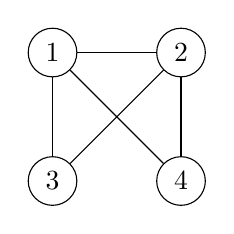
\begin{tikzpicture} [every node/.style={draw,circle}]
\node (a) {1};
\node (b) [right=of a] {2};
\node (c) [below=of a] {3};
\node (d) [right=of c] {4};
 
\draw[-](a)--(b);
\draw[-](a)--(c);
\draw[-](a)--(d);
\draw[-](b)--(d);
\draw[-](c)--(b);
\end{tikzpicture}     	
   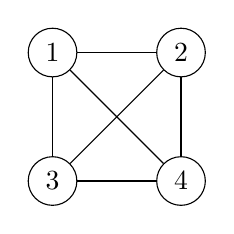
\begin{tikzpicture} [every node/.style={draw,circle}]
\node (a) {1};
\node (b) [right=of a] {2};
\node (c) [below=of a] {3};
\node (d) [right=of c] {4};
 
\draw[-](a)--(b);
\draw[-](a)--(c);
\draw[-](a)--(d);
\draw[-](b)--(d);
\draw[-](c)--(b);
\draw[-](c)--(d);
\end{tikzpicture}
  
  \item[2]
 All graphs of 3 vertices
 
     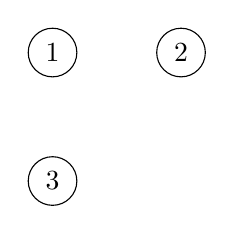
\begin{tikzpicture} [every node/.style={draw,circle}]
\node (a) {1};
\node (b) [right=of a] {2};
\node (c) [below=of a] {3};
\end{tikzpicture}
     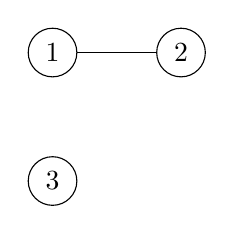
\begin{tikzpicture} [every node/.style={draw,circle}]
\node (a) {1};
\node (b) [right=of a] {2};
\node (c) [below=of a] {3};

\draw[-](a)--(b);
\end{tikzpicture} 
     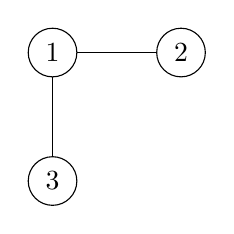
\begin{tikzpicture} [every node/.style={draw,circle}]
\node (a) {1};
\node (b) [right=of a] {2};
\node (c) [below=of a] {3};

\draw[-](a)--(b);
\draw[-](a)--(c);
\end{tikzpicture} 

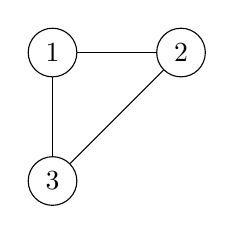
\begin{tikzpicture} [every node/.style={draw,circle}]
\node (a) {1};
\node (b) [right=of a] {2};
\node (c) [below=of a] {3};

\draw[-](a)--(b);
\draw[-](a)--(c);
\draw[-](b)--(c);
\end{tikzpicture}

\item[6]
\begin{enumerate}
  \item[a] Not Isomorpic, (a) contains 3 nodes of degree 2 and 3 nodes of degree
  4 while (b) contains 2 nodes of degree 2, 2 nodes of degree 3 and 2 nodes of
  degree 4. 
  \item[b] These are isomophic under the mapping
  (a,5),(b,6),(c,2),(d,1),(e,4),(f,3)
  \item[c] 
  asda
\end{enumerate}
\item[7]
7-11 is isomorphic to 25-30 under (30,7), (36,8), (28,9), (29,12), (27,11),
(25,10), 19-24 is isomorphic to 7-11 under (19,7),(22,8), (21,9),
(24,12),(23,10),(20,11). The others are not isomorphic. 
\item[10]
The first set is not isomorphic, the second set is under abcdef goes to 153426. 
\item[14] 
\begin{enumerate}
  \item[a]
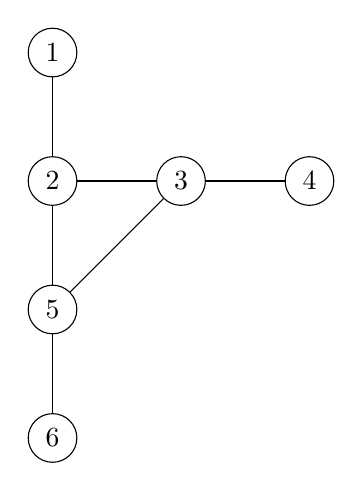
\begin{tikzpicture} [every node/.style={draw,circle}]
\node (a) {1};
\node (b) [below=of a] {2};
\node (c) [right=of b] {3};
\node (d) [right=of c] {4};
\node (e) [below=of b] {5};
\node (f) [below=of e] {6};

\draw[-](a)--(b);
\draw[-](b)--(c);
\draw[-](c)--(d);
\draw[-](b)--(e);
\draw[-](c)--(e);
\draw[-](e)--(f);
\end{tikzpicture}
  	
  \item[b]
  Impossible, the sum of the degrees is odd. 
  \item[c]
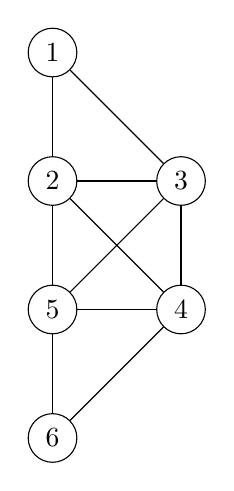
\begin{tikzpicture} [every node/.style={draw,circle}]
\node (a) {1};
\node (b) [below=of a] {2};
\node (c) [right=of b] {3};
\node (d) [below=of c] {4};
\node (e) [below=of b] {5};
\node (f) [below=of e] {6};

\draw[-](a)--(b);
\draw[-](a)--(c);
\draw[-](b)--(c);
\draw[-](b)--(d);
\draw[-](c)--(d);
\draw[-](b)--(e);
\draw[-](c)--(e);
\draw[-](d)--(e);
\draw[-](d)--(f);
\draw[-](e)--(f);
\end{tikzpicture}  
\end{enumerate}
\item[1.3.3]
Since 2(19) = (sum of degrees) = 38. The maximum possible number of vertices if each has at least degree 3 is 12. If there were 13 vertices then at least one vertex would have to have degree 2.
\item[1.3.4]
In this case G must have an odd number of vertices. Then in the complement each vertex with an odd degree in G also has an odd degree in the complement of G. Therefore all but one vertex has an odd degree in the complement of G and one vertex has an even degree, the same as in G. 

\item[1.3.7]
Suppose all vertices of a G have degree p, where p is odd, the sum of all the degrees of all the vertices is np, where n is the number of vertices in G. By theorem 1, the sum of the degrees is equal to twice the number of edges, in which case, np = 2e, where e is the number of edges in G. Then e = $\frac{n}{2}p$, therefore e is a multiple of p. 
\item[1.3.8]
Since there are 13 teams in a conference, with each playing exactly 11
in-conference games there needs to be 143 games held. Since a game must consist
of two teams, and its impossible to divide 143 by 2, there can be no graph for
this configuration, meaning that at least 1 team will have to play 12 games in
order for the others to play 11. 
\end{enumerate}
\end{document}
